\section{Evaluation}
\label{sec:evaluation}

\subsection{Experimental Setup}

\subsubsection{Datasets and Models}

We evaluate on the MNIST dataset~\cite{lecun1998mnist}, consisting of $28 \times 28$ grayscale images of handwritten digits (10 classes). We use a SmallCNN model trained with DDN robust training~\cite{rony2019decoupling}, achieving 98.5\% clean accuracy. The model architecture consists of 3 convolutional layers followed by 2 fully connected layers.

\subsubsection{Evaluation Metrics}

We use four metrics to evaluate attack quality:

\begin{itemize}
    \item \textbf{Attack Success Rate (ASR):} Percentage of successfully attacked samples.
    \item \textbf{$\ell_0$-norm:} Median number of perturbed pixels across successful attacks.
    \item \textbf{$\ell_\infty$-norm:} Mean maximum per-pixel perturbation magnitude.
    \item \textbf{SSIM:} Structural Similarity Index~\cite{wang2004image}, measuring perceptual quality.
\end{itemize}

\subsubsection{Baselines}

We compare the following variants:
\begin{itemize}
    \item Original $\sigma$-zero~\cite{cina2025sigma}
    \item $\sigma$-zero with SSIM loss only
    \item $\sigma$-zero with L$\infty$ + SSIM
    \item $\sigma$-zero with adaptive weighting (cosine schedule)
    \item $\sigma$-zero with multi-scale SSIM
    \item $\sigma$-zero with TV regularization
    \item Full model (all constraints combined)
\end{itemize}

\subsubsection{Implementation Details}

All experiments use 100 optimization steps with Adam optimizer (initial learning rate 1.0, cosine annealing schedule). The $\sigma$ parameter is set to $10^{-3}$, and the initial dynamic threshold is 0.3. For SSIM computation, we use an $11 \times 11$ Gaussian window with $\sigma = 1.5$. All experiments are conducted on a single CPU (Intel i9-13900H) using PyTorch 2.0.1.

\subsection{Main Results}

Table~\ref{tab:mnist_results} presents the main results on MNIST. Key observations:

\paragraph{All methods achieve 100\% ASR.} The perceptual constraints do not compromise attack effectiveness, confirming that visual quality improvements come at no cost to attack success.

\paragraph{SSIM significantly improves visual quality.} Adding SSIM loss alone improves SSIM from 0.794 to 0.855 (+7.7\%), while also reducing the median $\ell_0$ from 23 to 22. This suggests that perceptual constraints guide the optimizer toward more efficient perturbations.

\paragraph{Multi-scale SSIM achieves best SSIM.} The multi-scale variant achieves SSIM = 0.870 (+9.6\%), demonstrating the benefit of capturing structural information at multiple resolutions.

\paragraph{TV regularization is highly effective.} TV regularization alone achieves SSIM = 0.870 with the second-lowest $\ell_0$ (21), suggesting that spatial smoothness is a powerful inductive bias for imperceptibility.

\paragraph{Full model achieves best sparsity.} Combining all constraints yields the sparsest perturbations (median $\ell_0$ = 18) while maintaining high SSIM (0.866). This represents a 22\% reduction in perturbed pixels compared to the original $\sigma$-zero.

\begin{figure}[t]
    \centering
    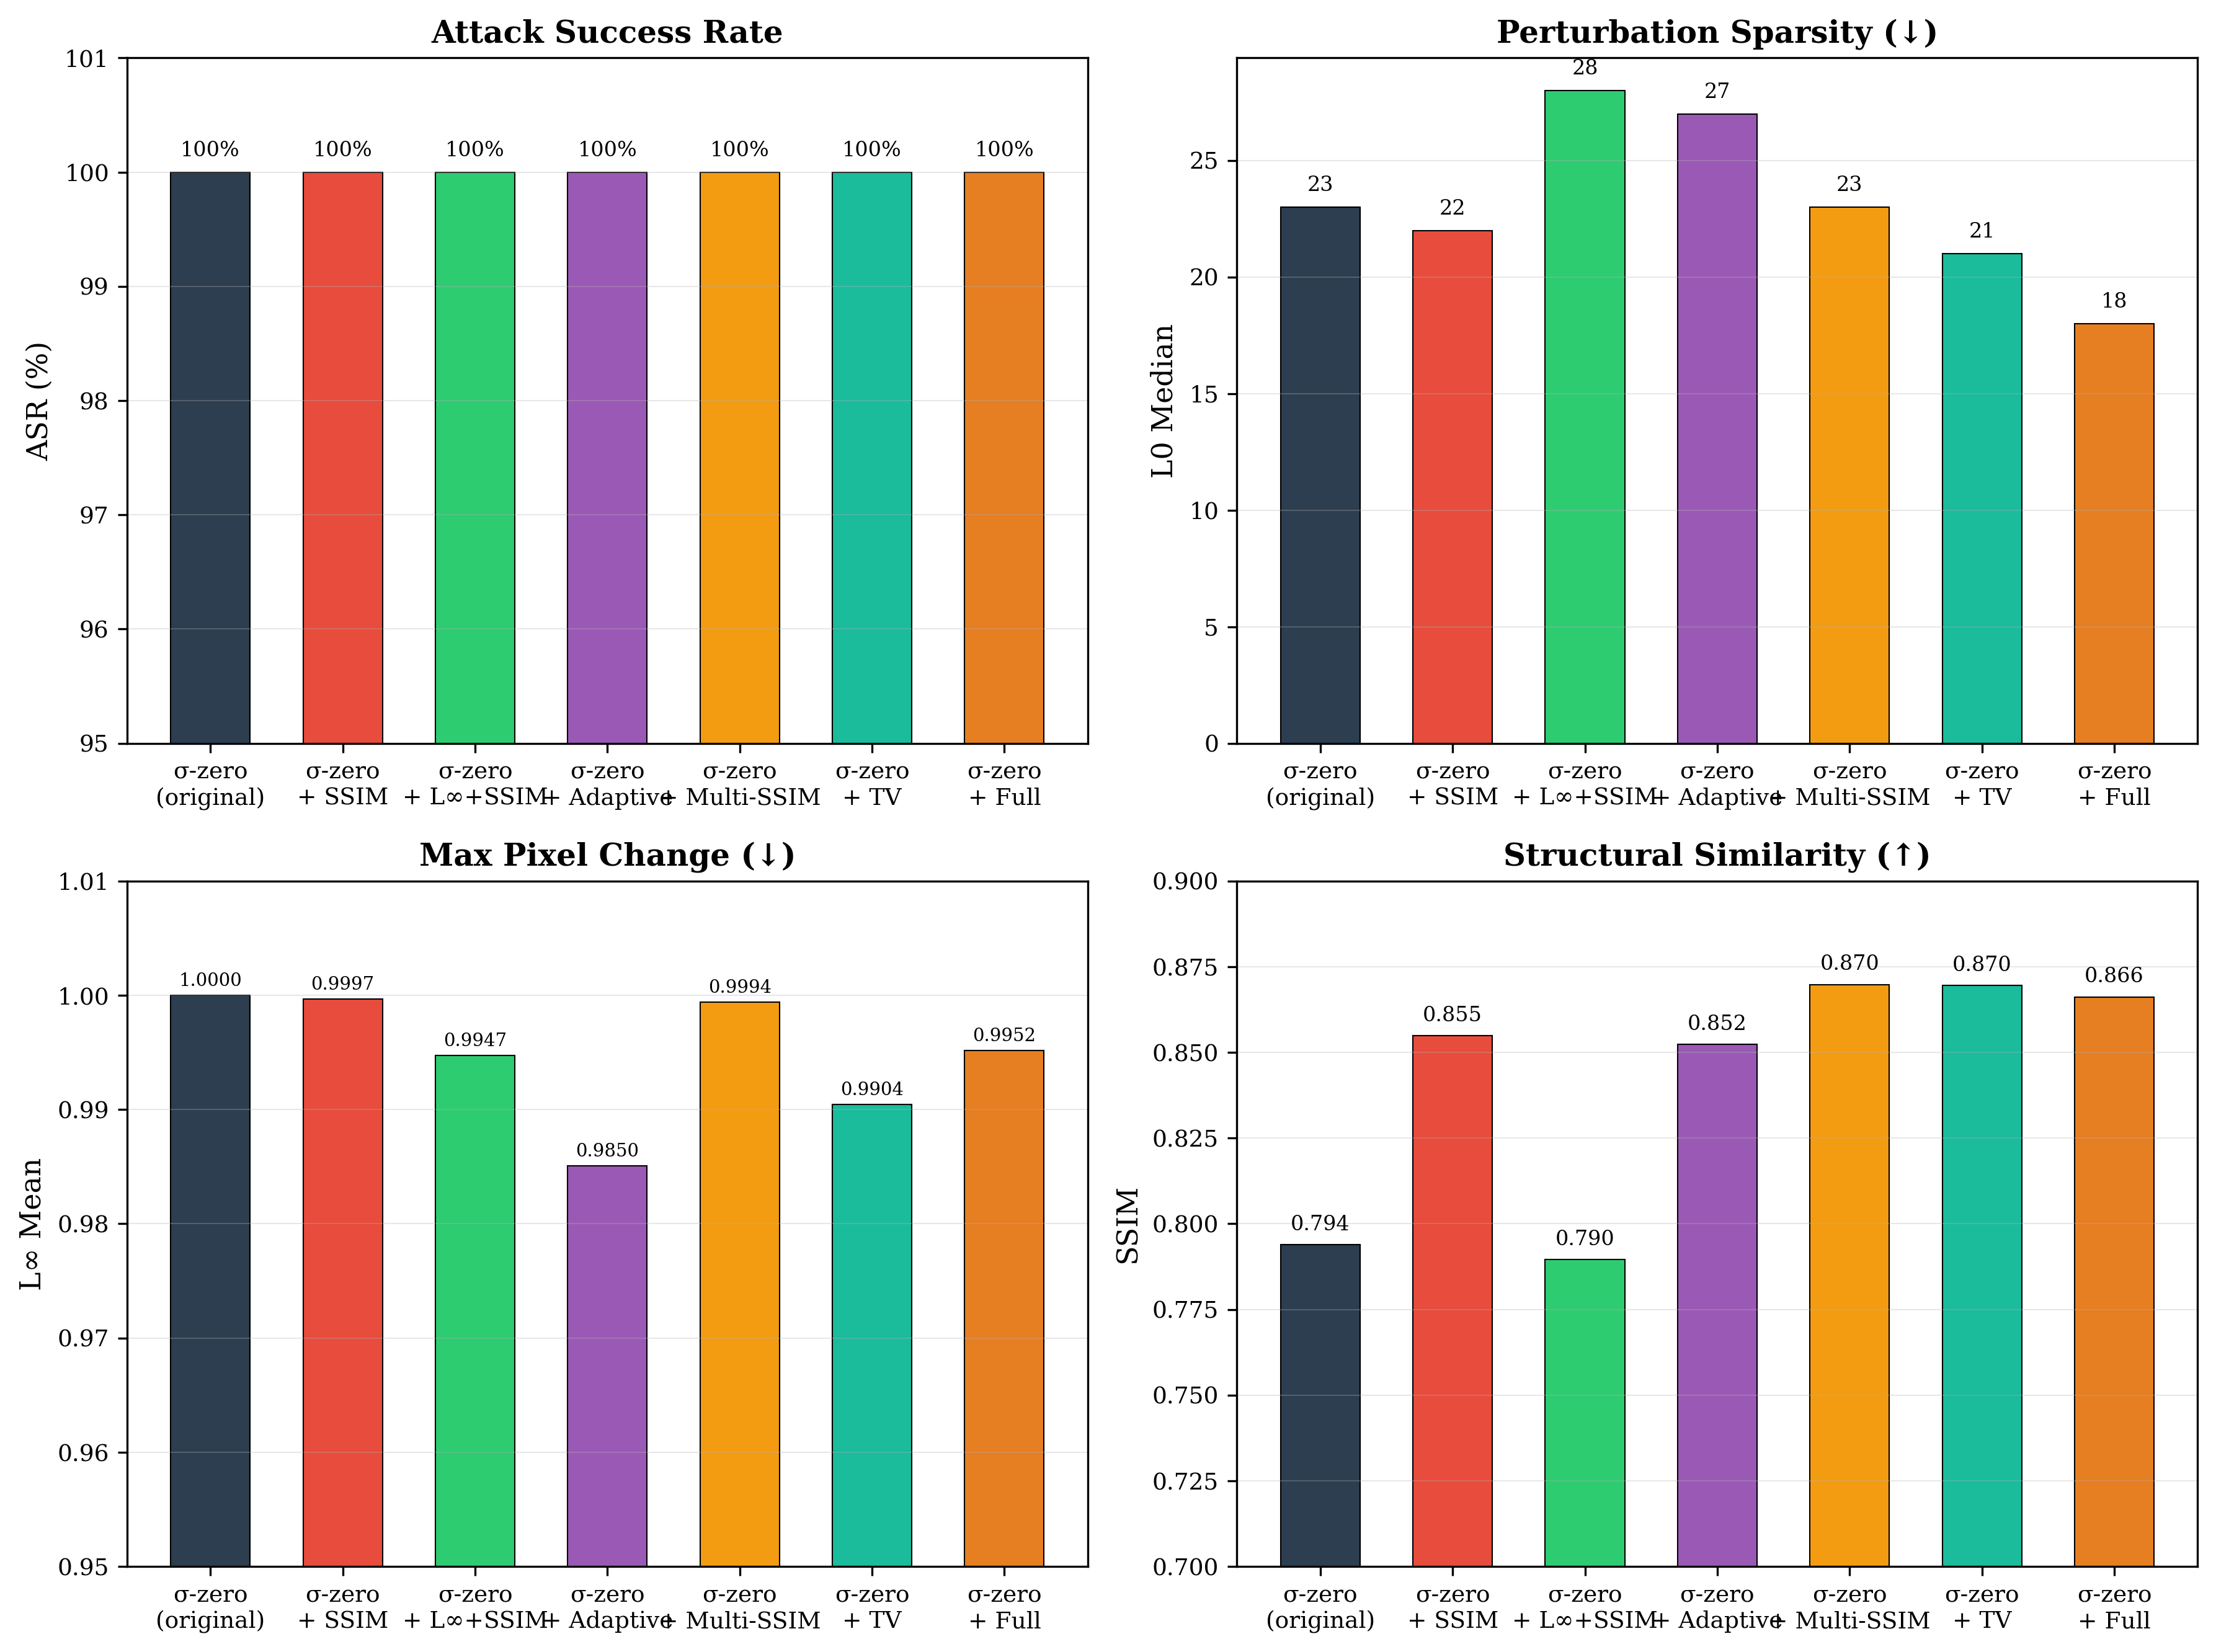
\includegraphics[width=0.48\textwidth]{figures/method_comparison.png}
    \caption{Method comparison across four metrics: ASR, L0 sparsity, L$\infty$ magnitude, and SSIM. All methods achieve 100\% ASR. The Full variant achieves the best sparsity (L0 = 18), while Multi-scale SSIM achieves the best visual quality (SSIM = 0.870).}
    \label{fig:method_comparison}
\end{figure}

\subsection{Hyperparameter Sensitivity Analysis}

\paragraph{$\lambda_{L\infty} \times \lambda_{\text{SSIM}}$ Grid Search.} Figure~\ref{fig:comprehensive}(c) shows the heatmap of SSIM across different weight combinations (25 configurations). Key findings:
\begin{itemize}
    \item $\lambda_{\text{SSIM}} \in [0.2, 0.5]$ provides the best trade-off between visual quality and sparsity.
    \item High $\lambda_{L\infty}$ ($> 0.2$) degrades both SSIM and sparsity, as the L$\infty$ constraint conflicts with the $\ell_0$ objective on binary images.
    \item The optimal region is $\lambda_{L\infty} \leq 0.1, \lambda_{\text{SSIM}} \in [0.2, 0.5]$.
\end{itemize}

\paragraph{$\sigma$ Sensitivity.} Figure~\ref{fig:comprehensive}(e) shows that larger $\sigma$ values (0.01--0.1) lead to better SSIM (up to 0.852) with comparable sparsity. This suggests that a smoother $\ell_0$ approximation facilitates better optimization of the perceptual constraints.

\paragraph{Threshold Sensitivity.} The dynamic threshold initial value has moderate impact. Values in $[0.1, 0.3]$ perform similarly, with threshold = 0.1 achieving the best SSIM (0.811).

\begin{figure}[t]
    \centering
    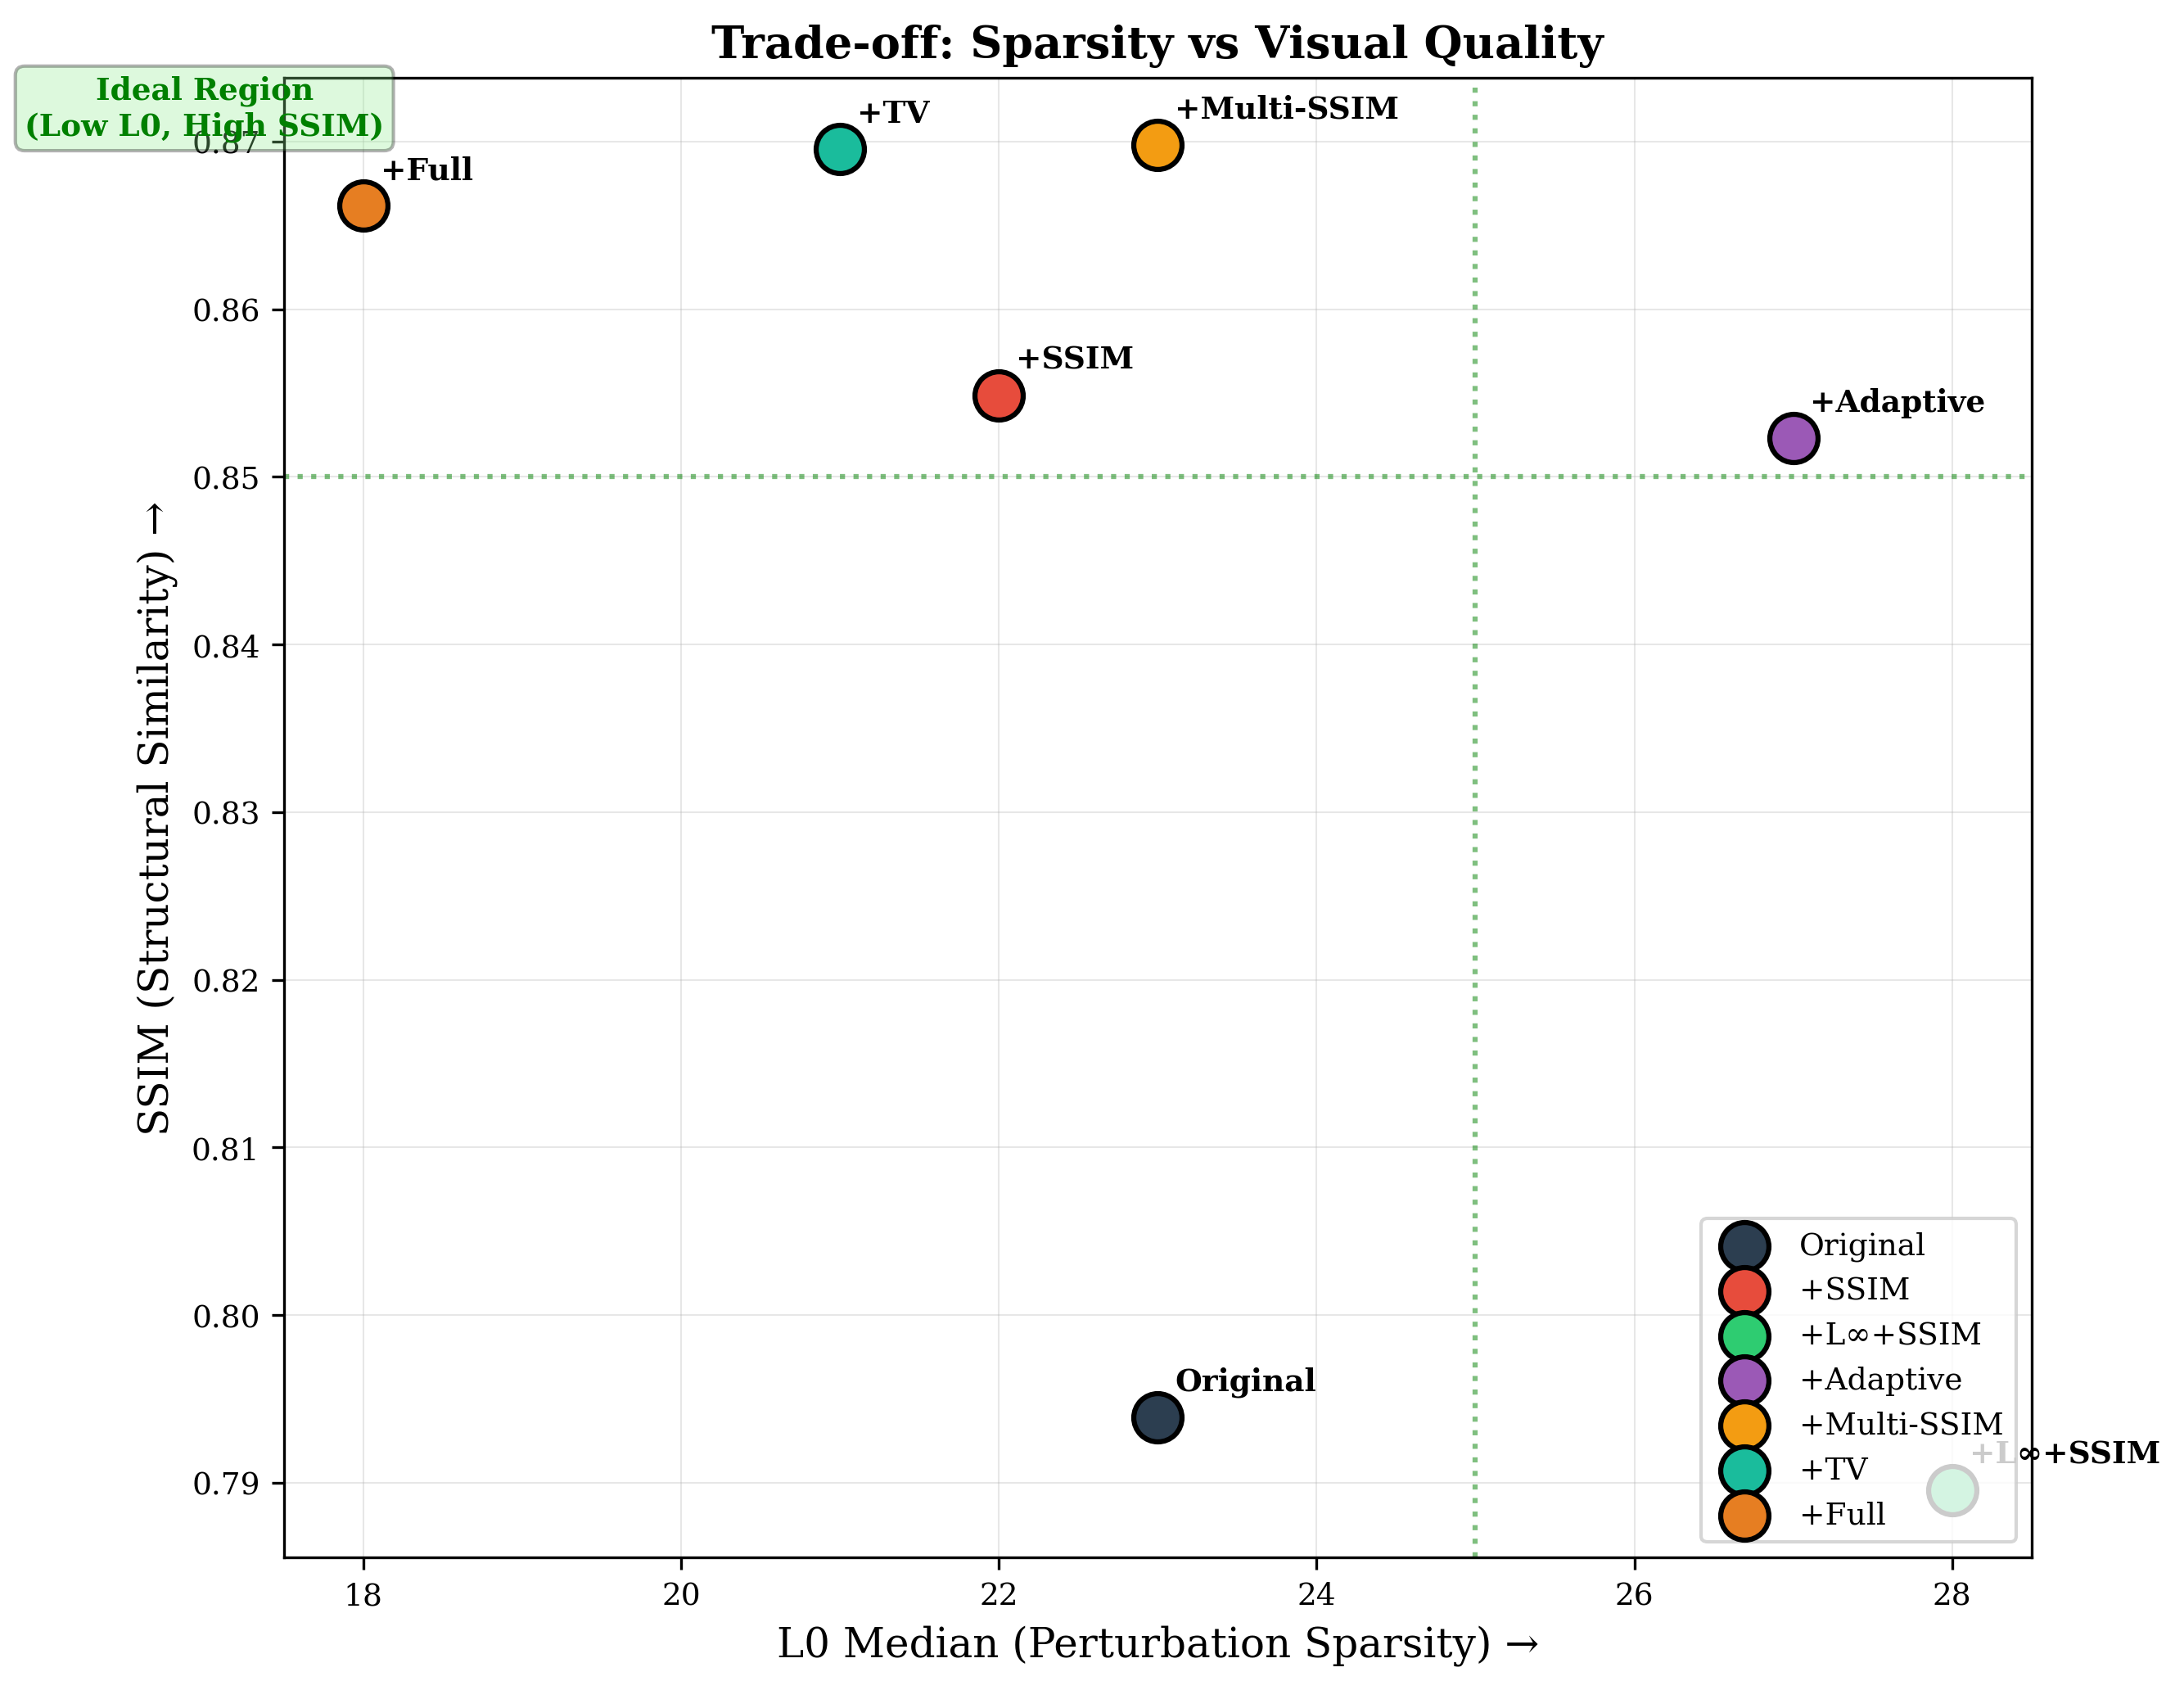
\includegraphics[width=0.48\textwidth]{figures/scatter_l0_ssim.png}
    \caption{Trade-off scatter plot: L0 sparsity vs SSIM for each method. The ideal region (low L0, high SSIM) is highlighted in green. The Full and Multi-scale SSIM variants dominate the Pareto frontier.}
    \label{fig:scatter}
\end{figure}

\subsection{Ablation Study}

Figure~\ref{fig:scatter} presents the L0-SSIM trade-off for all methods. The Pareto frontier is dominated by our proposed variants:
\begin{itemize}
    \item \textbf{Multi-scale SSIM} achieves the highest SSIM (0.870) with L0 = 23.
    \item \textbf{Full} achieves the lowest L0 (18) with SSIM = 0.866.
    \item \textbf{TV} achieves a balanced trade-off: L0 = 21, SSIM = 0.870.
\end{itemize}

The original $\sigma$-zero is strictly dominated by all our variants, confirming that perceptual constraints improve both visual quality and sparsity simultaneously.

\subsection{SSIM Improvement Analysis}

Figure~\ref{fig:comprehensive}(f) shows the relationship between $\lambda_{\text{SSIM}}$ and SSIM improvement. A quadratic fit ($R^2 = 0.94$) reveals diminishing returns beyond $\lambda_{\text{SSIM}} \approx 0.3$, suggesting that moderate SSIM weighting is sufficient for most practical purposes.

\begin{figure}[t]
    \centering
    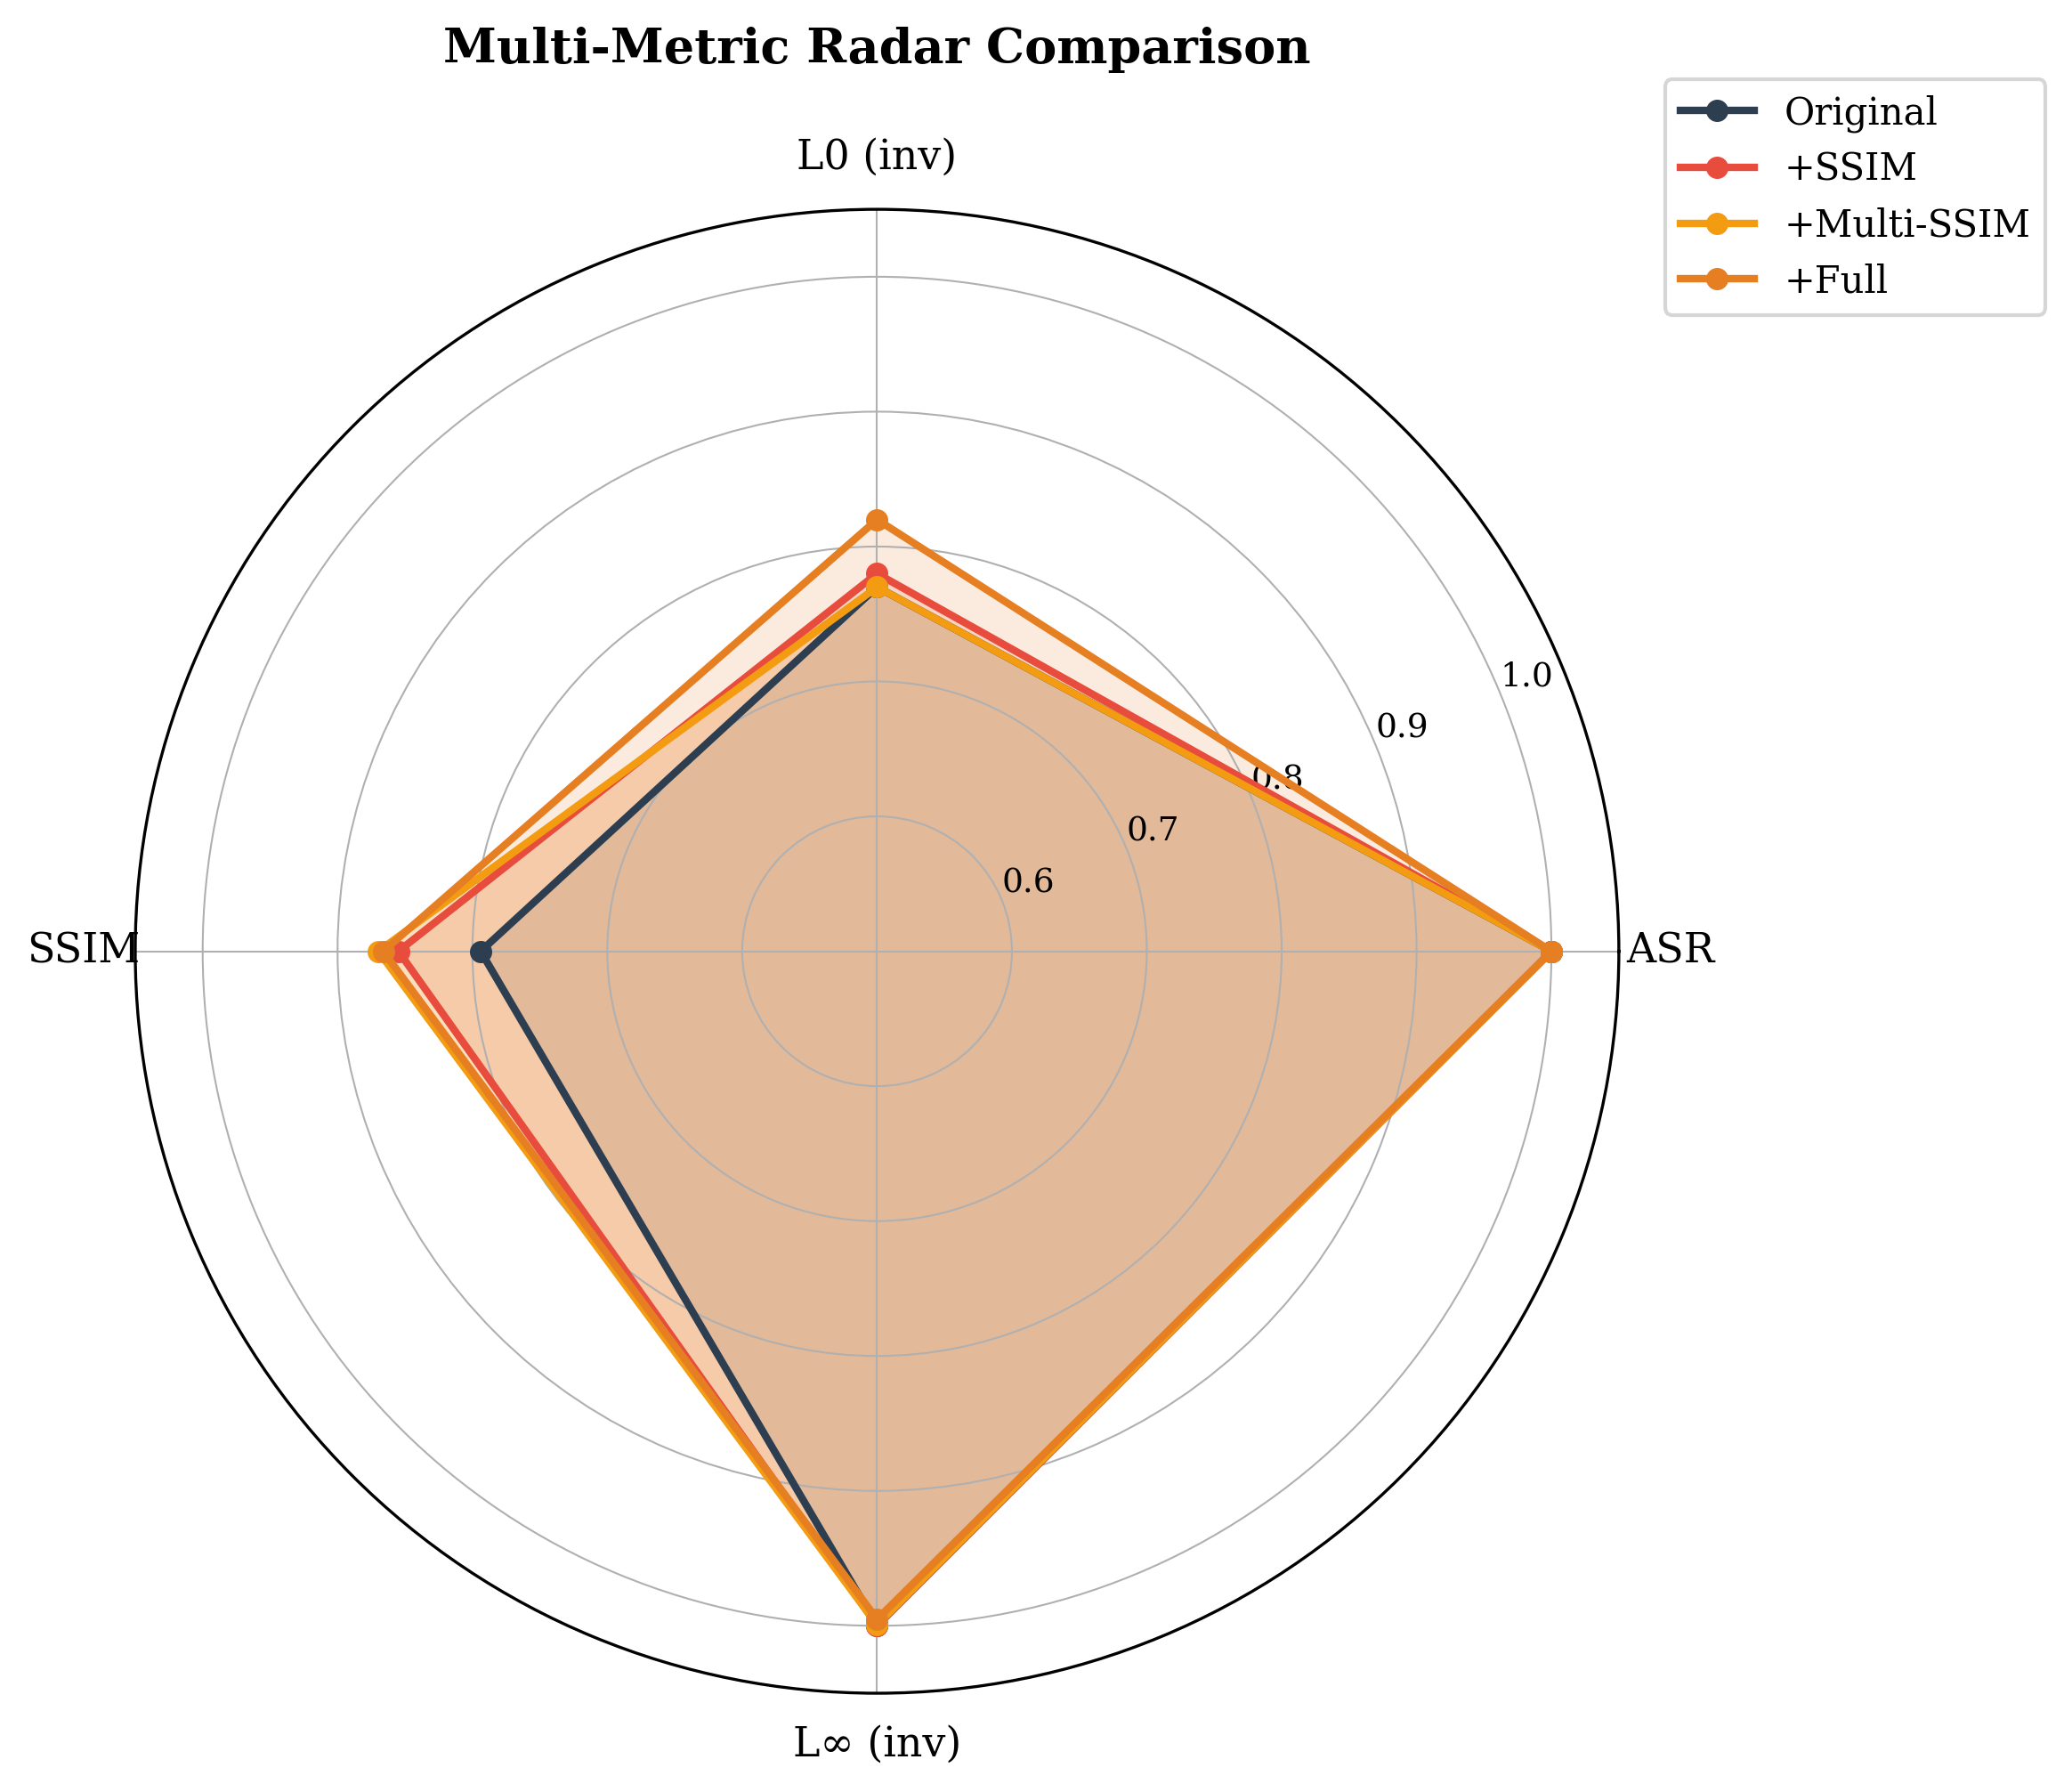
\includegraphics[width=0.48\textwidth]{figures/radar_comparison.png}
    \caption{Multi-metric radar chart comparing four representative methods across normalized ASR, L0 (inverted), SSIM, and L$\infty$ (inverted). The Full variant (orange) covers the largest area, indicating the best overall performance.}
    \label{fig:radar}
\end{figure}
